%% ----------------------------------------------------------------
%% Thesis.tex -- MAIN FILE 
%% Use the "Thesis" style, based on the ECS Thesis style by Steve Gunn
%% Revised by Qiang Yang
%% ---------------------------------------------------------------- 

% Set up the document
\documentclass[a4paper, 11pt, twoside]{Thesis} 


%----------packages----------------
\usepackage{amsmath,amssymb,amsfonts}
\usepackage{mathptmx}
\usepackage[ruled,linesnumbered]{algorithm2e}
\usepackage{multirow}
\usepackage{wrapfig}
\graphicspath{{Figures/}} % Location of the graphics files (set up for graphics to be in PDF format)
\usepackage{subfig}
\captionsetup{labelfont=rm,figurename=Figure} %FIGURE->Figure
\captionsetup[subfloat]{labelfont=rm,labelformat=simple} % (A)->(a)
\renewcommand{\thesubfigure}{(\alph{subfigure})} % Fig. 3.3a -> Fig.3.3(a)
\usepackage{gensymb} % \degree
\usepackage{graphbox}
\usepackage{libertine}
\usepackage[square, numbers, comma, sort&compress]{natbib}  % Use the "Natbib" style for the references in the Bibliography
\usepackage{verbatim}  % Needed for the "comment" environment to make LaTeX comments
\usepackage{float} % To keep figures in place
\hypersetup{urlcolor=black, % url
citecolor=violet, % citation
linkcolor=violet, % table of contents, inner color
colorlinks=true,  
pdfborder = {0 0 0}}  % Colours hyperlinks in blue
% Define enumerated description lists
\usepackage{enumitem}
\usepackage{kantlipsum}
%------------------------------------

%----------new commands--------------
\renewcommand{\bibname}{Reference}
\newcommand{\todo}[1]{\textcolor{red}{TODO: #1}\PackageWarning{TODO:}{#1!}}
\newcommand{\update}[1]{\textcolor{blue}{#1}}
\newcommand{\rev}[1]{\textcolor{red}{#1}} 
\newcommand{\etal}{\textit{et al}.}
\newcommand{\ie}{\textit{i}.\textit{e}.}
\newcommand{\eg}{\textit{e}.\textit{g}.}
\newcommand{\etc}{\textit{etc}.}
\newcommand{\bits}[1]{\texttt{#1}}
\newcommand{\cmd}[1]{\texttt{#1}}
\newcommand{\code}[1]{\texttt{#1}}
\renewcommand\chaptermark[1]{\markboth{\chaptername\ \thechapter. #1}{}}
\renewcommand\sectionmark[1]{\markright{\thesection. #1}}
%--------------------------------------

%-------------control-------------------
\addtolength{\oddsidemargin}{-18pt} % left margin of odd
\addtolength{\evensidemargin}{18pt} % left margin of even
\newcounter{descriptcount}
\newcounter{descriptcount2}
\newlist{enumdescript}{description}{2}
\setlist[enumdescript,1]{%
  before={\setcounter{descriptcount}{0}%
          \renewcommand*\thedescriptcount{\arabic{descriptcount}.}}
  ,font=\bfseries\stepcounter{descriptcount}\thedescriptcount~
}
\setlist[enumdescript,2]{%
  before={\setcounter{descriptcount2}{0}%
          \renewcommand*\thedescriptcount{\roman{descriptcount2}.}}
  ,font=\bfseries\stepcounter{descriptcount2}\thedescriptcount~
}
% reduce the word break between lines
% \tolerance=1
% \emergencystretch=\maxdimen
% \hyphenpenalty=10000
% \hbadness=10000
%---------------------------------------


\makeatother


%% ------------Document begins---------------------------
\begin{document}

%% ---Cover page---------------
%% -------------
% Cover page
\pagestyle{empty}

\vfill\vfill\vfill\vfill\vfill\vfill\vfill\vfill\null

\begin{center}

\vfill

{\LARGE\MakeUppercase{\textbf{PolyU Ph.D. Thesis Latex Template}} \par}

% Delete this line when submitting the final version
\textbf{\textit{\large Initial Submission for Examination Purpose}}
\vfill

{\LARGE \textbf{Name} \par}

\vspace{20pt}

{\LARGE \textbf{PhD} \par}

\vfill
\vfill

{\LARGE \textbf{The Hong Kong Polytechnic University} \par}

\vspace{20pt}

{\LARGE \textbf{2022}}
\vfill\vfill
\end{center}

\let\cleardoublepage\clearpage  % clear empty page

%%-------title page------------
% For changes in supervisor, degree type, research group, etc. please change the Thesis.cls file

\frontmatter      % Begin the book's numbering; frontpage
%\pagenumbering{arabic}

% Set up the Title Page
\title{PolyU Ph.D. Thesis Latex Template}

\authors  {\texorpdfstring
            {\href{mailto:emailAddress@connect.polyu.hk}{Name}}
            {Author's Name}
            }
\addresses  {\groupname\\\deptname\\\univname}  % Do not change this here, instead these must be set in the "Thesis.cls" file, please look through it instead
\date       {24 June 2022}
\subject    {}
\keywords   {}

\maketitle

%% ------------format settings ---------

\setstretch{1.5}  % It is better to have smaller font and larger line spacing than the other way round

% Define the page headers using the FancyHdr package and set up for one-sided printing
\fancyhead{}  % Clears all page headers and footers
\rhead{\thepage}  % Sets the right side header to show the page number
\lhead{}  % Clears the left side page header
\pagestyle{fancy}  % Finally, use the "fancy" page style to implement the FancyHdr headers

%% ------------Declaration Page----------
% Declaration Page required for the Thesis, your institution may give you a different text to place here
\Declaration{

% \addtocontents{toc}{\vspace{1em}}  % Add a gap in the Contents, for aesthetics
\vspace{\stretch{0.1}}

I hereby declare that this thesis is my own work and that, to the best of my knowledge and belief, it reproduces no material previously published or written, nor material that has been accepted for the award of any other degree or diploma, except where due acknowledgement has been made in the text.
 

  \vspace{\stretch{0.1}}
  \begin{flushleft}
    \begin{tabular}{c c c c l}%{l p{0.5in} p{1in} p{0.5in} l}
      & & {
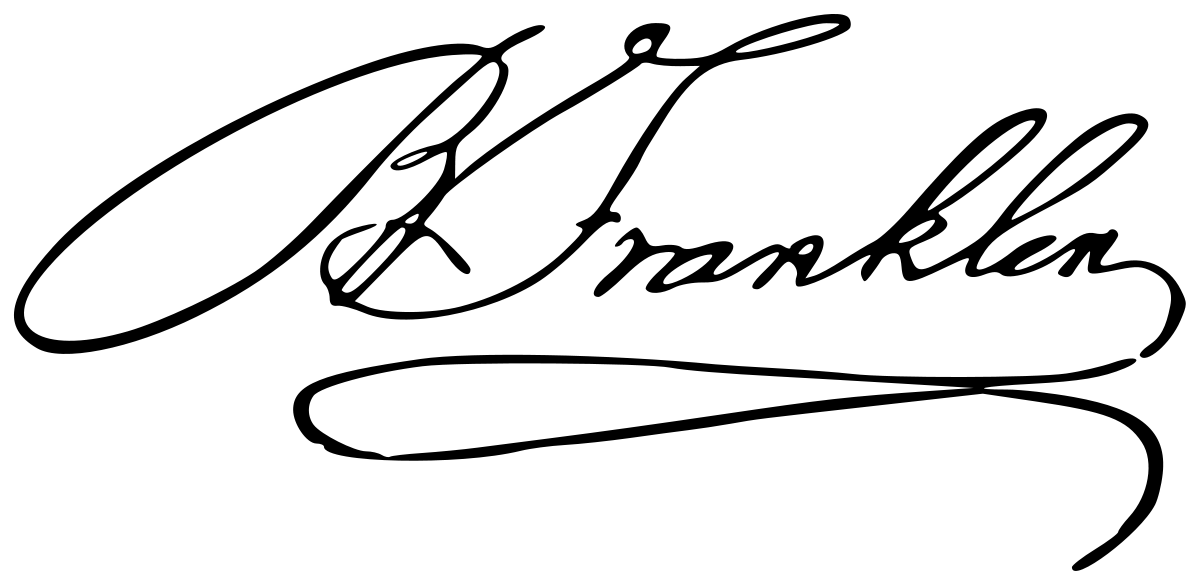
\includegraphics[width=0.2\textwidth]{Figures/Benjamin_Franklin.png}
} & & (Signed) \\
      \cline{1-4}\\
      & & Your name  & & (Name of student) \\
      \cline{1-4}\\
    \end{tabular}
  \end{flushleft}
  \vspace{\fill}
  
}
\clearpage  % Declaration ended, now start a new page


%% -------------
% add a empty page
% \pagestyle{empty}
% \vfill\vfill\vfill\vfill\vfill\vfill\null

% \clearpage
%% --------------


%%--------- The Abstract Page---------------------
\addtotoc{Abstract}  % Add the "Abstract" page entry to the Contents
\abstract{
%\addtocontents{toc}{\vspace{1em}}  % Add a gap in the Contents, for aesthetics

Abstract goes here.

\kant[1-3]


} % abstract end
\clearpage  % Abstract ended, start a new page

%%----------Publication Page----------------------
\publications{

\begin{enumerate}[label={[\arabic*]}]

    \item \textbf{Qiang Yang}, “PolyU Ph.D. Thesis Latex Template”, github.com, June 26, 2022.
    

\end{enumerate}
}
\clearpage


%-----------The Acknowledgements page-------------
\acknowledgements{
Acknowledgements go here.

\kant[1-2]

}

\clearpage  % End of the Acknowledgements


%% ---------Add Table of Content-------------------

\pagestyle{fancy}  %The page style headers have been "empty" all this time, now use the "fancy" headers as defined before to bring them back

\lhead{\emph{Contents}}  % Set the left side page header to "Contents"
\tableofcontents  % Write out the Table of Contents

%% ---------List of Figures and Tables-------------
\lhead{\emph{List of Figures}}  % Set the left side page header to "List if Figures"
\listoffigures  % Write out the List of Figures
\let\cleardoublepage\clearpage % clear the blank page

\lhead{\emph{List of Tables}}  % Set the left side page header to "List of Tables"
\listoftables  % Write out the List of Tables

%% ---------Abbreviations-----------------------------
\setstretch{1.5}  % Set the line spacing to 1.5, this makes the following tables easier to read
% \clearpage  % Start a new page
% \lhead{\emph{Abbreviations}}  % Set the left side page header to "Abbreviations"
% \listofsymbols{ll}  % Include a list of Abbreviations (a table of two columns)
% {
% \textbf{Acronym} & \textbf{W}hat (it) \textbf{S}tands \textbf{F}or \\
% % Abbreviations go here
% }



%% ---------Text format--------------------------------
\mainmatter	  % Begin normal, numeric (1,2,3...) page numbering
\pagestyle{fancy}  % Return the page headers back to the "fancy" style
\fancyhf{}
\fancyhead[OL]{\rightmark}
\fancyhead[OR]{\thepage}
\fancyhead[EL]{\thepage}
\fancyhead[ER]{\leftmark}


%%---------Thesis text----------------------------------


\chapter{Introduction} \label{Chap: introduction}

This is a latex template for Ph.D. thesis in The Hong Kong Polytechnic University. It can be also used for other universities or degrees.

\section{Commands}

This is an example for renew commands, \eg, we can use \textbackslash eg to generate \eg. The same thing goes to \etc.

We can use \textbackslash rev\{\} to mark your text: \rev{revised text}. 


\section{Citation}

This is an example for citation \cite{pan2012investigation}.

\section{Figures}


This is a figure, as shown in \fref{fig:figure}.


 \begin{figure}[t]
     \centering
     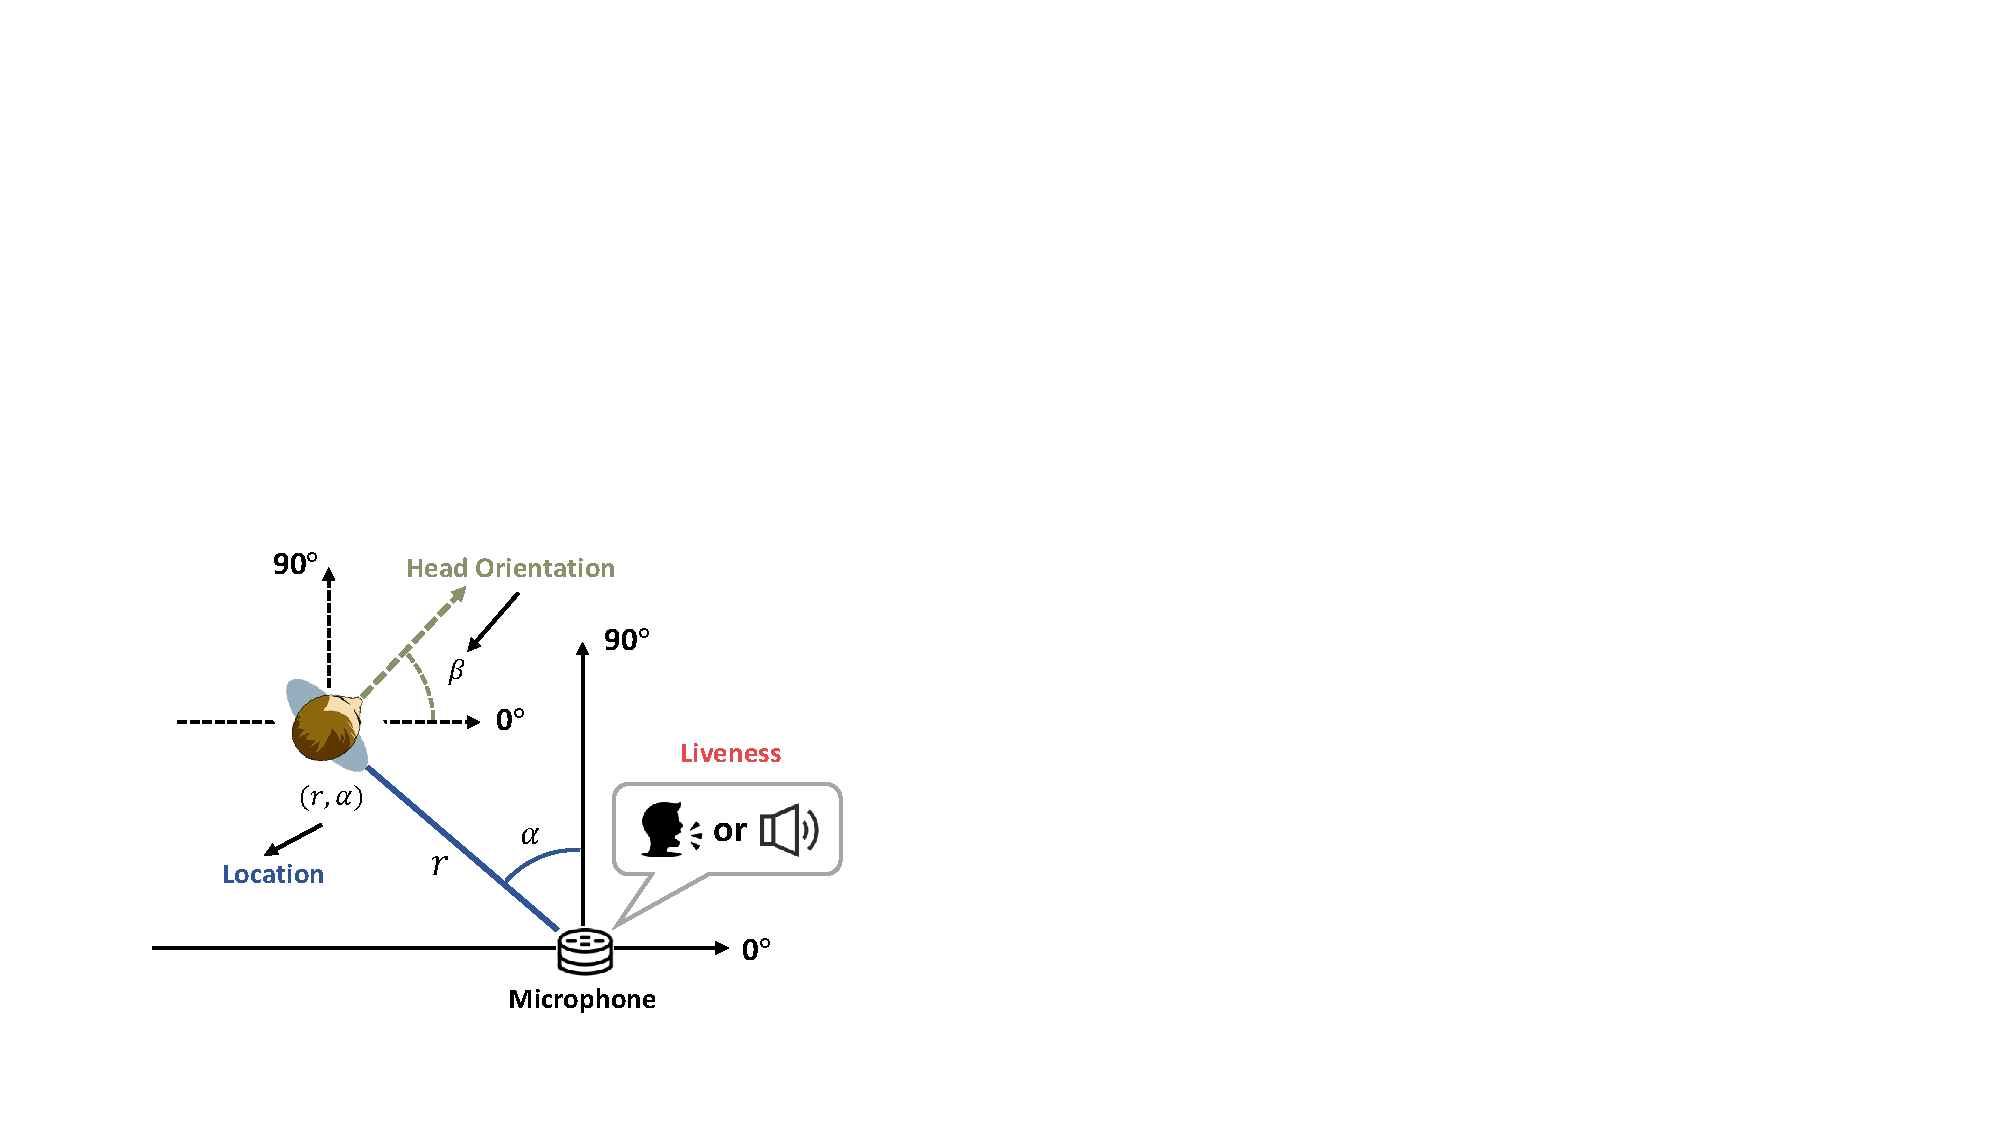
\includegraphics[width=0.5\textwidth]{Figures/Illustration.pdf}
     \caption{Illustration of a figure.}
     \label{fig:figure}
 \end{figure}

Figure \ref{fig:subfigure} shows an example of subfigures (\fref{fig:subfigure1} and \fref{fig:subfigure2}).


\begin{figure}[t]
\centering
\subfloat[Subfigure 1]{
		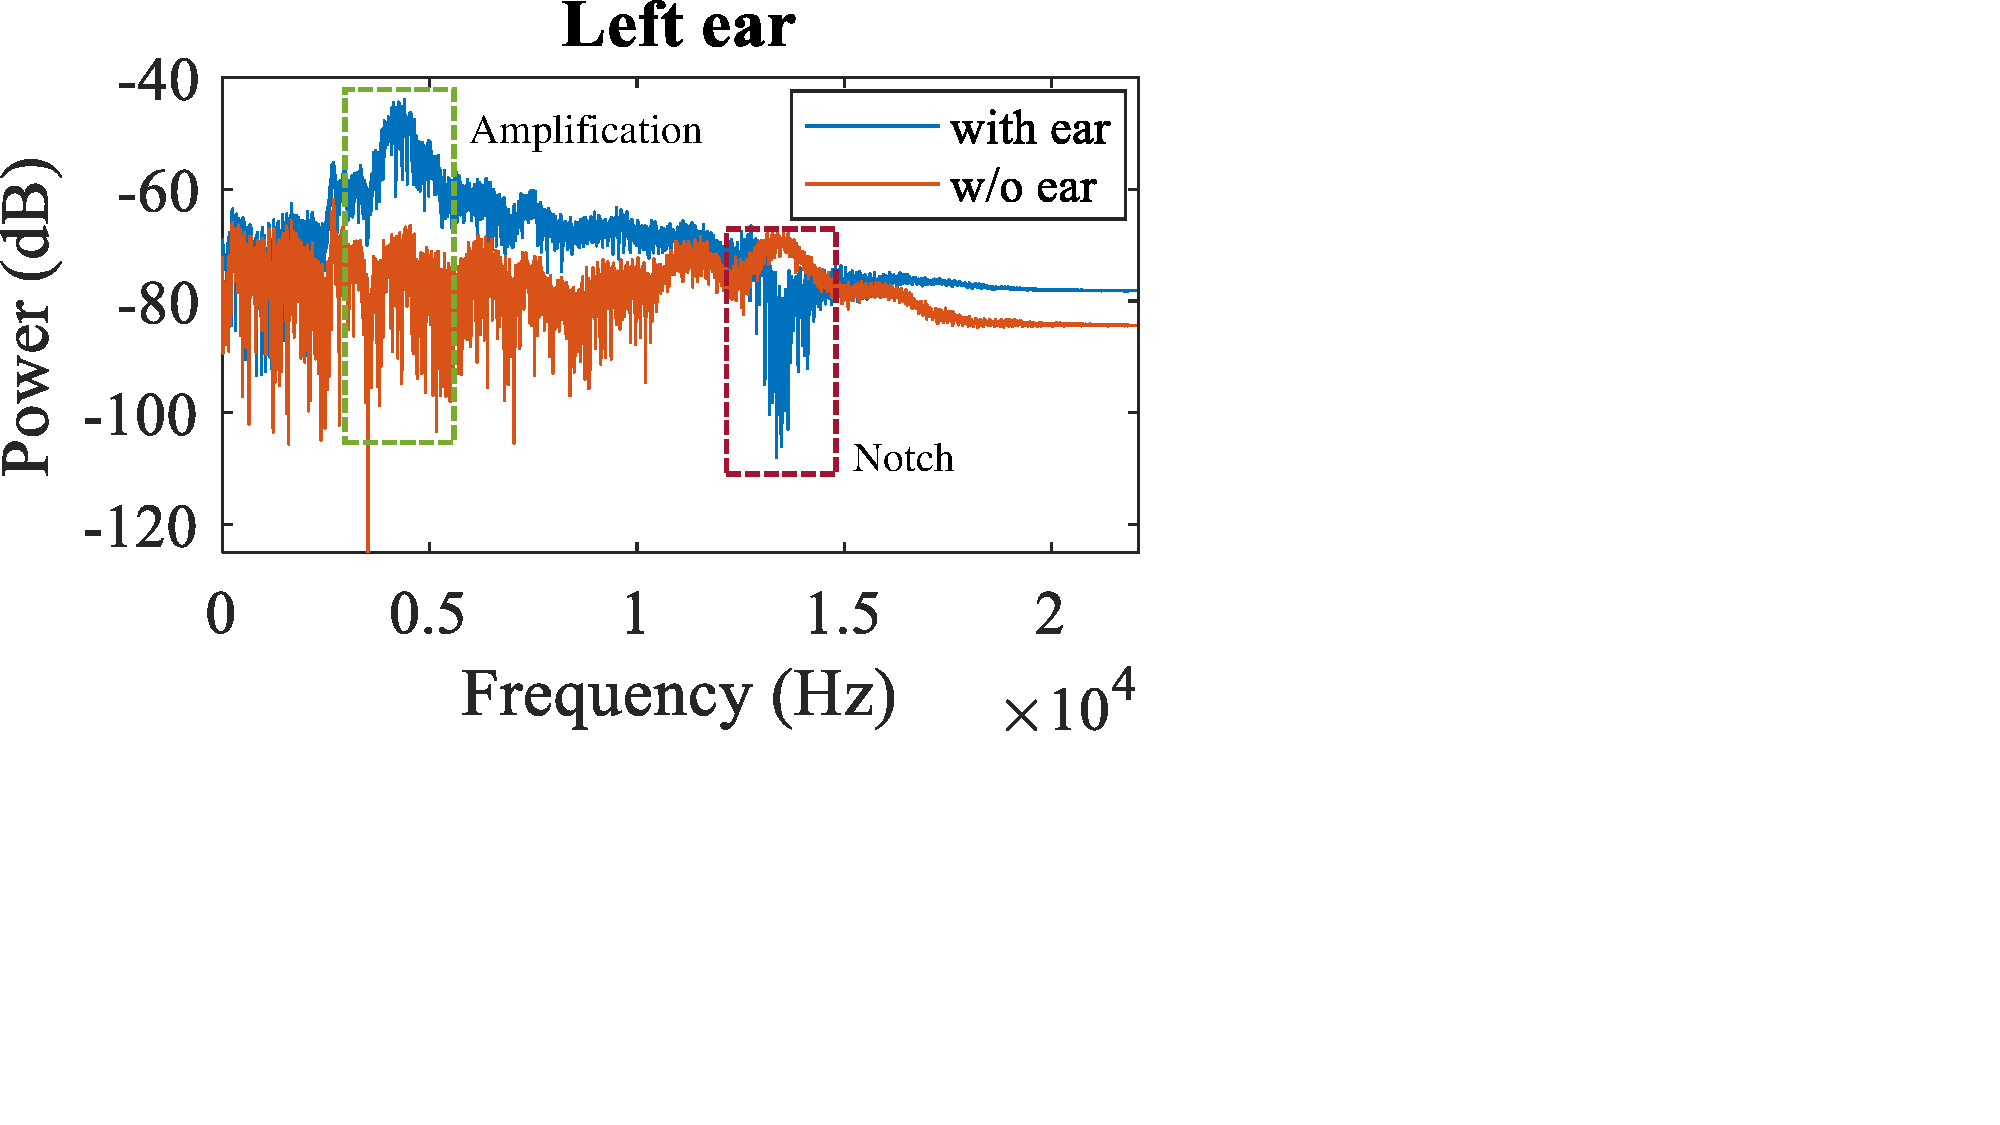
\includegraphics[width=0.45\columnwidth]{Figures/fr_ear_left.pdf} 
		\label{fig:subfigure1}
	}
\subfloat[Subfigure 2]{
		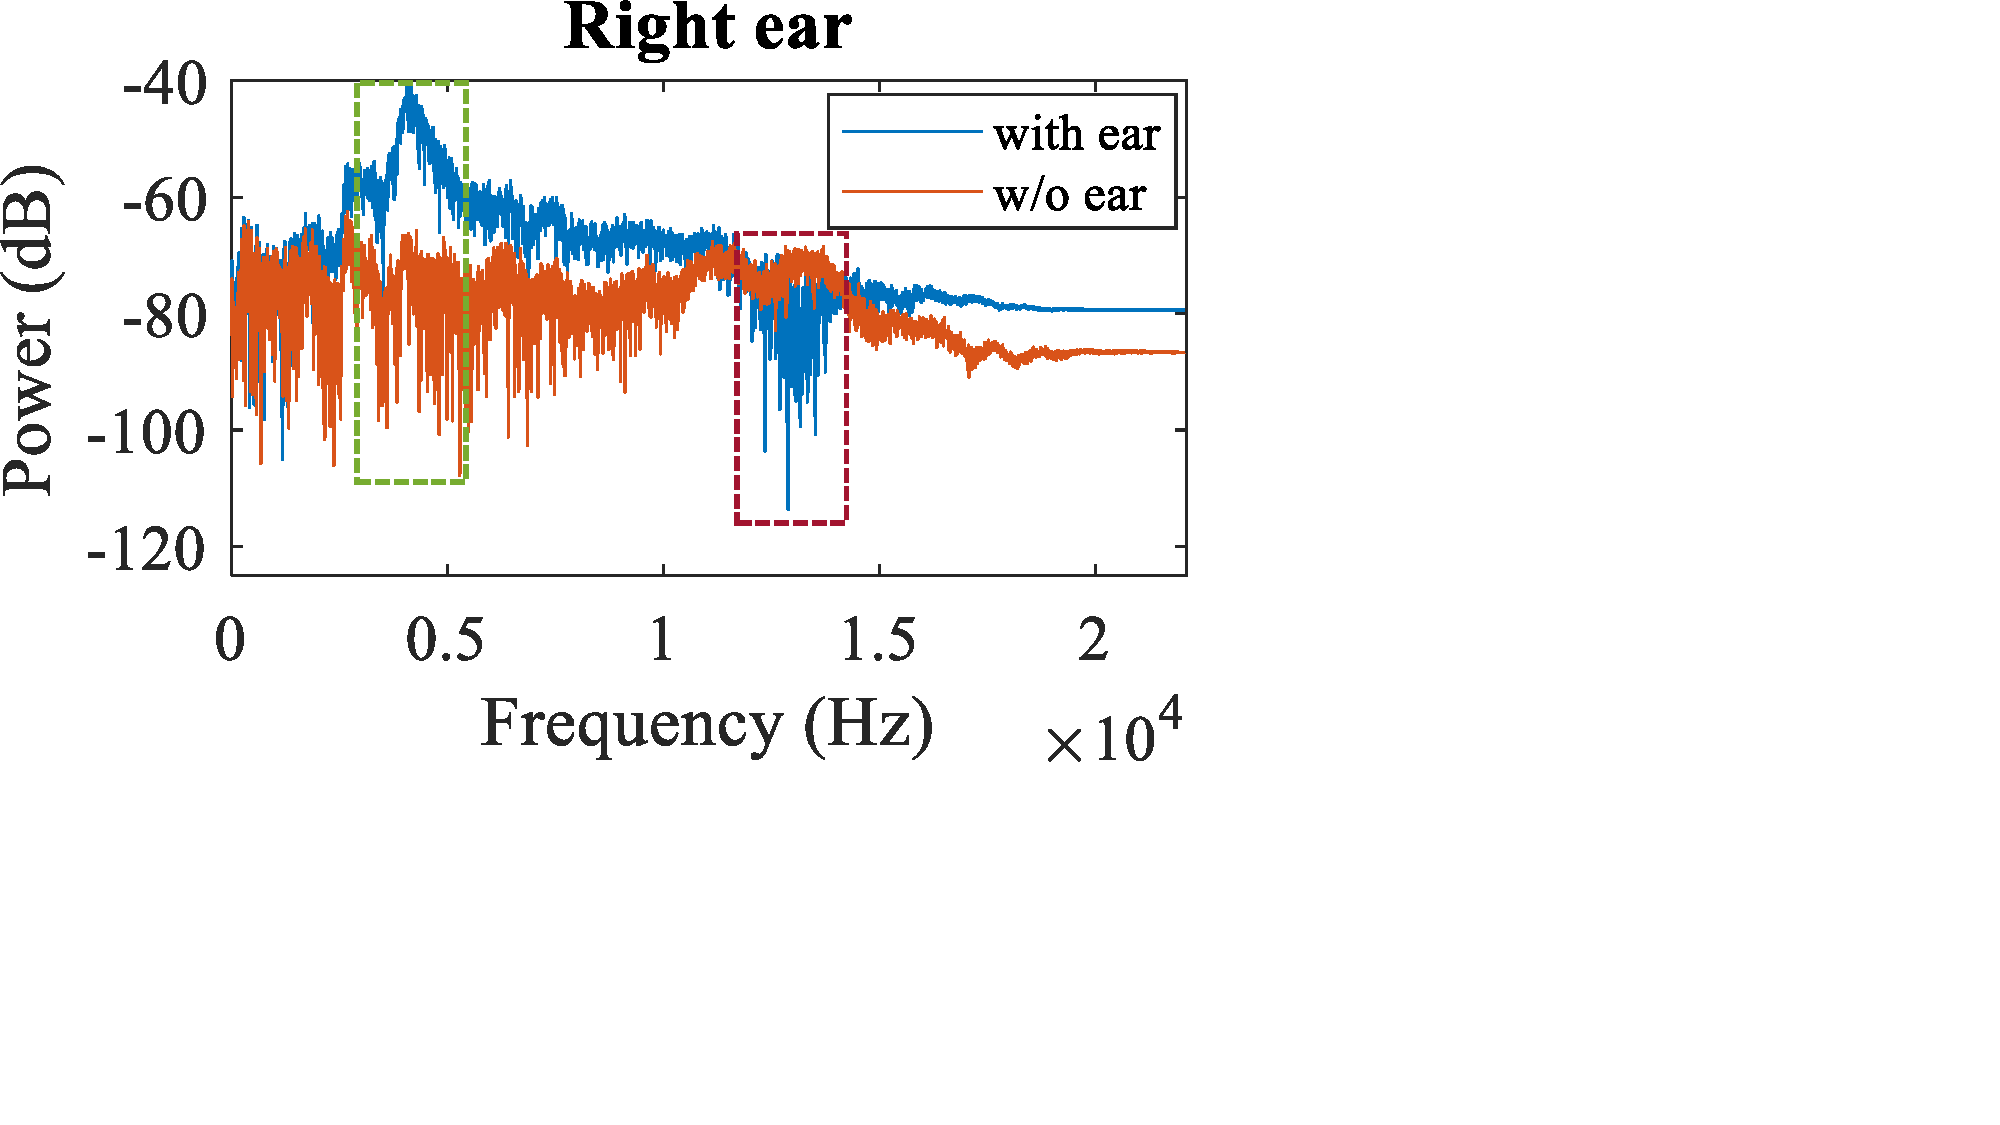
\includegraphics[width=0.45\columnwidth]{Figures/fr_ear_right.pdf}
		\label{fig:subfigure2}
	}
\caption{Frequency response with and without ears.}
\label{fig:subfigure}
\end{figure}


This is an example for the minipage (\fref{fig:minipage1} and \fref{fig:minipage2}).

\begin{figure}[t]
\begin{minipage}{0.48\linewidth}
        \centering
		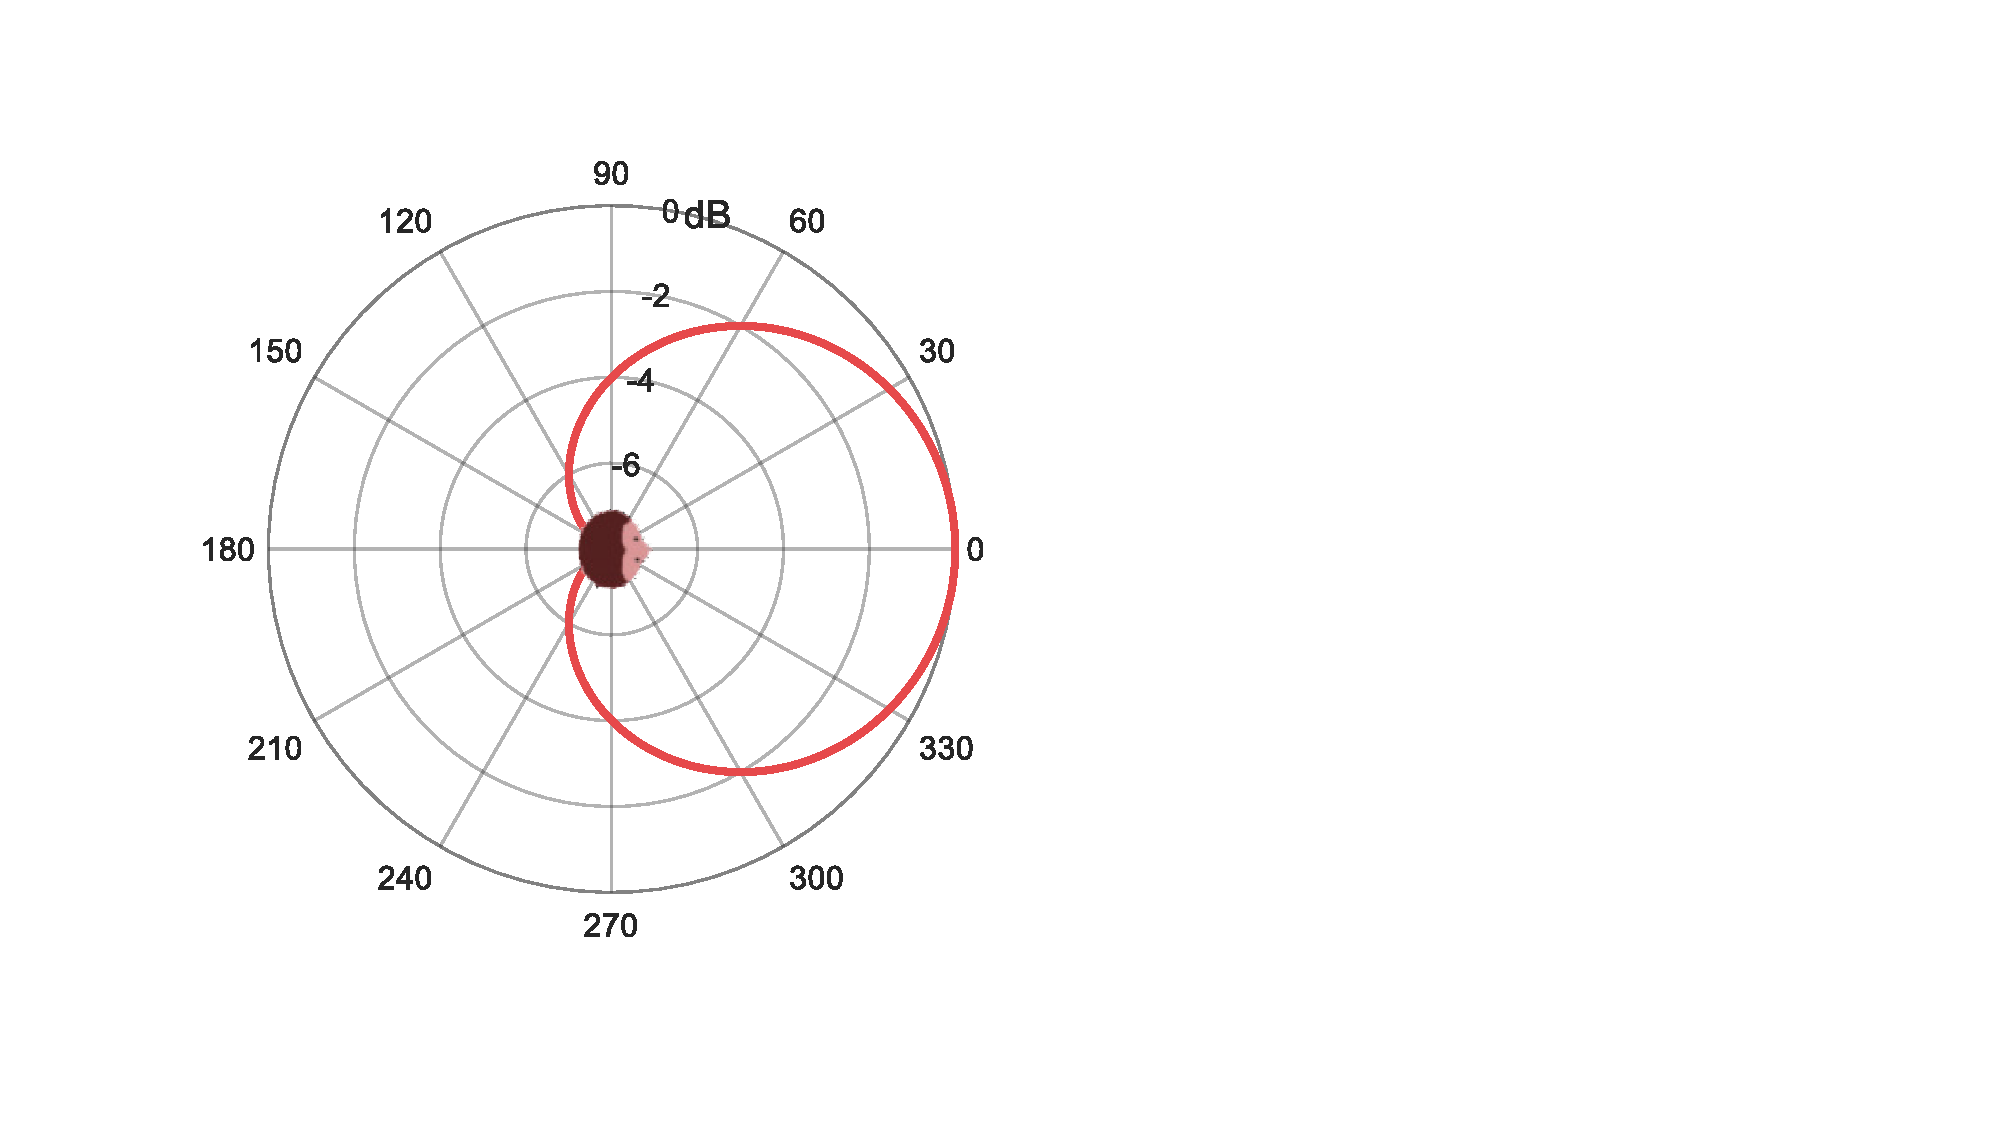
\includegraphics[width=0.58\columnwidth]{Figures/OE_cardioid.pdf}
		\caption{Minipage 1.}
		\label{fig:minipage1}
\end{minipage}
\hspace{5pt}
\begin{minipage}{0.48\linewidth}
        \centering
		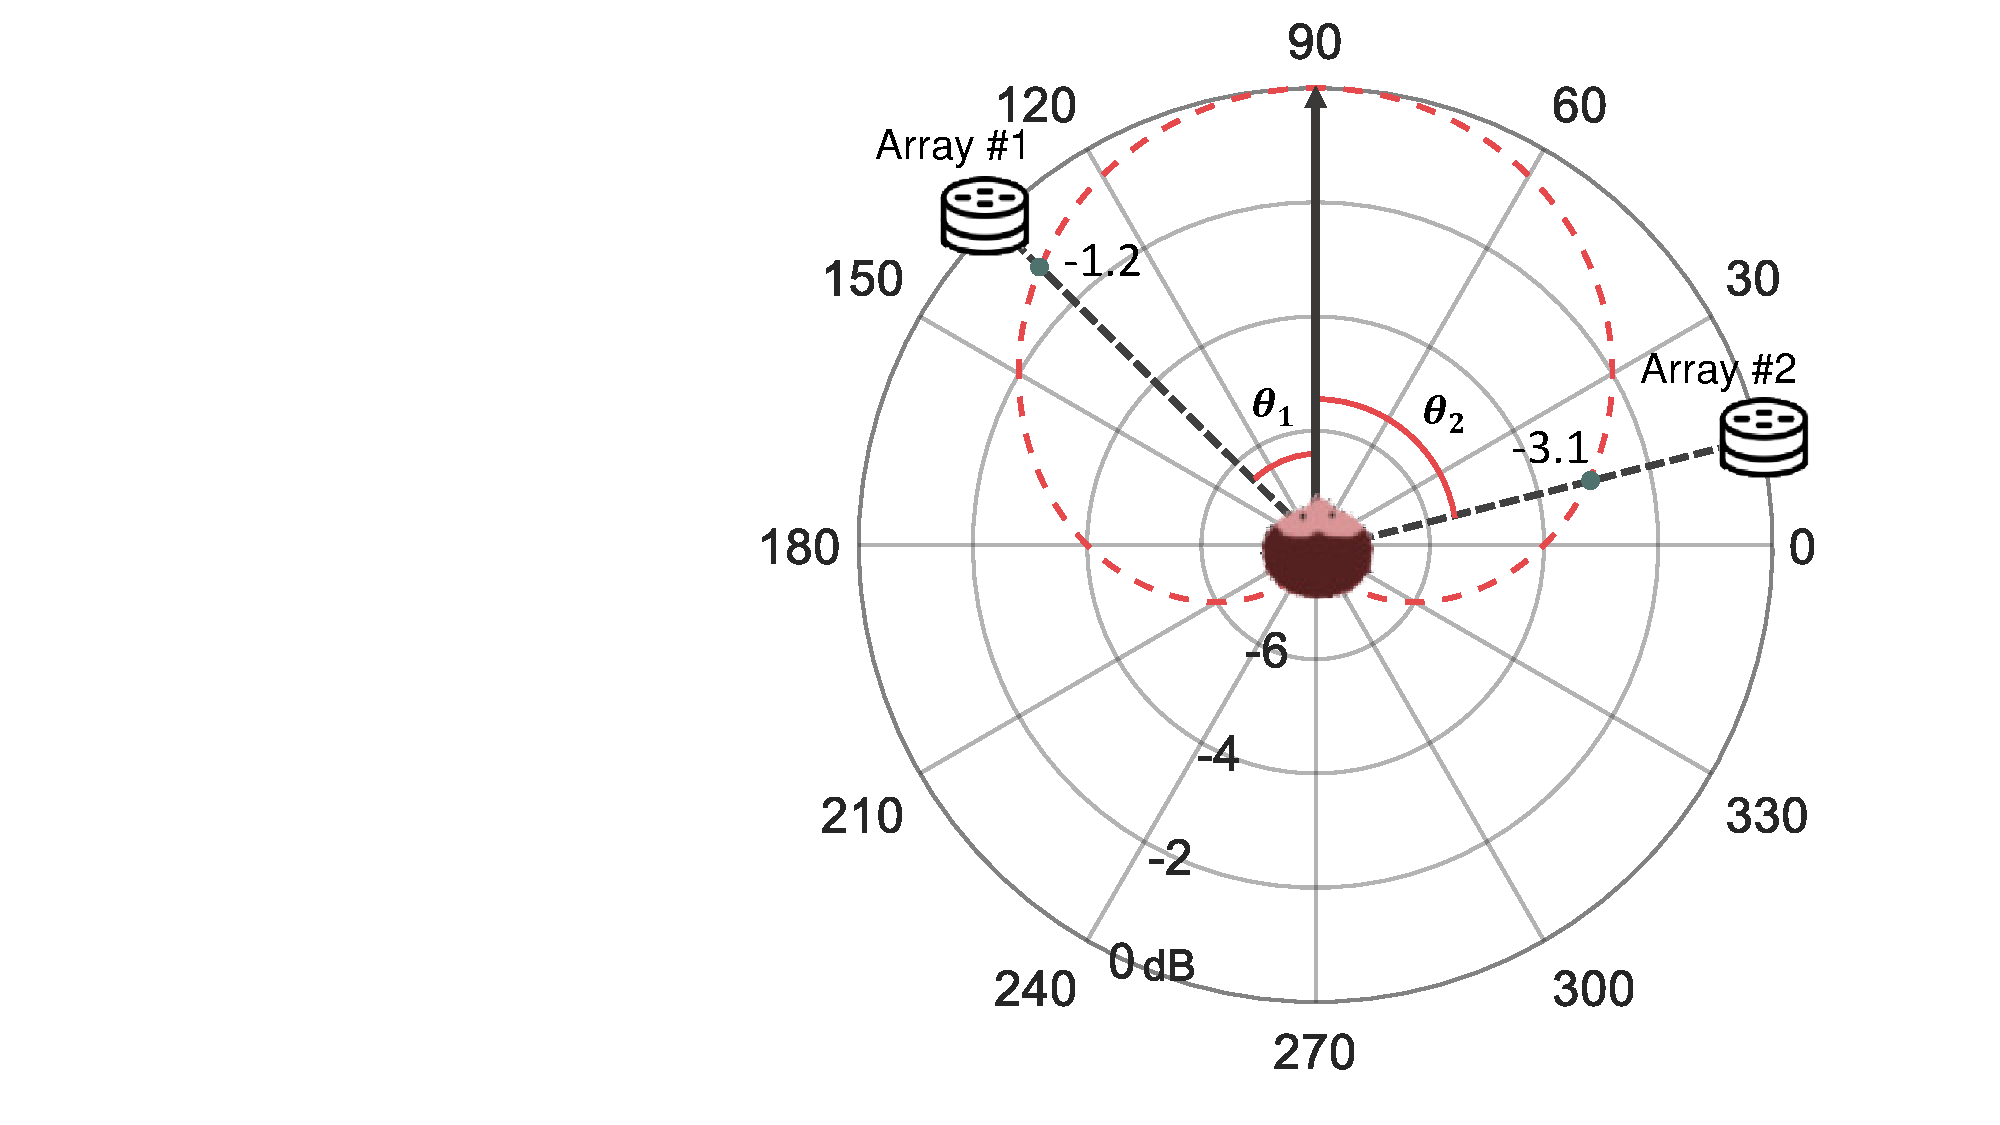
\includegraphics[width=0.58\columnwidth]{OE_sameDisDiffDeg.pdf}
		\caption{Minipage 2.}
		\label{fig:minipage2}
\end{minipage}
\end{figure}

\section{Table}


A table example is shown in \tref{tab:table}. It is a three-line table.


\begin{table}[t]
\renewcommand{\arraystretch}{1.1}
\centering
\caption{PolyU rankings.}
\begin{tabular}{ccccc}
\toprule
Rankings &
  \begin{tabular}[c]{@{}c@{}}QS \\ World University\end{tabular} &
  \begin{tabular}[c]{@{}c@{}}QS \\ Asia University \end{tabular} &
  \begin{tabular}[c]{@{}c@{}}THE \\ World University \end{tabular} &
  \begin{tabular}[c]{@{}c@{}}THE \\ Asia University\end{tabular} \\ \midrule
2022 &
  66 &
  25 &
  91 &
  15 \\ 
2021 &
  75 &
  25 &
  129 &
  23 \\ \bottomrule
\end{tabular}
\vspace{10pt}
\label{tab:table}
\end{table}

\section{Examples}


\kant[1-3] 


\addtocontents{toc}{\vspace{2em}}  % Add a gap in the Contents, for aesthetics
\backmatter % End the book's numbering; backpage

%% --------Reference-------------------------------------
\label{Bibliography}
\fancyhf{}
\fancyhead[OL]{\emph{Reference}}
\fancyhead[OR]{\thepage}
\fancyhead[EL]{\thepage}
\fancyhead[ER]{\emph{Reference}}

% Reference style
\bibliographystyle{ACM-Reference-Format}
\bibliography{mybibfile}  

\end{document}  % The End
%% ----------------------------------------------------------------